% !TEX program = xelatex
\documentclass[UTF8,11pt,a4paper,fontset=fandol]{ctexart}
% 主文件用 \documentclass[UTF8,11pt,a4paper,fontset=fandol]{ctexart}。
% 通用视觉底座。教学顺序、助教台词、署名与题目由主文件决定。
\usepackage[left=23mm,right=23mm,top=19mm,bottom=18mm,headheight=15pt,headsep=6mm,footskip=9mm]{geometry}
\usepackage{amsmath,amssymb,graphicx,xcolor,fancyhdr,tabularx,booktabs,tikz}
\usetikzlibrary{calc,arrows.meta,angles,quotes,intersections,positioning}

\definecolor{BrickRed}{HTML}{8B4739}
\definecolor{RoyalBlue}{HTML}{355E51}
\definecolor{handoutink}{HTML}{253630}
\definecolor{handoutmuted}{HTML}{58665E}
\setlength{\parindent}{0pt}
\setlength{\parskip}{5pt plus 1pt}
\linespread{1.08}
\setlength{\emergencystretch}{3em}

\newcommand{\HandoutHeader}[3][]{%
  \pagestyle{fancy}\fancyhf{}
  \fancyhead[L]{\small #2}\fancyhead[R]{\small #3}
  \fancyfoot[L]{\scriptsize\fangsong #1}\fancyfoot[R]{\small\thepage}
  \renewcommand{\headrulewidth}{.3pt}}
\newcommand{\HandoutLesson}[2]{%
  \par{\small\heiti\color{BrickRed}#1}\par\vspace{3pt}
  {\fontsize{21}{27}\selectfont\heiti\bfseries #2}\par
  \textcolor{BrickRed}{\rule{\linewidth}{.7pt}}\par}
\newcommand{\HandoutBlock}[1]{\par\vspace{4pt}{\large\heiti\bfseries #1}\par}
\newcommand{\HandoutNote}[1]{\par{\fangsong\fontsize{10.3}{15}\selectfont\color{handoutmuted}#1\par}}
\newcommand{\HandoutBox}[1]{%
  \par\noindent\begingroup\setlength{\fboxsep}{8pt}%
  \colorbox{BrickRed!9}{\parbox{\dimexpr\linewidth-16pt\relax}{#1}}\endgroup\par}
\newcommand{\HandoutHighlight}[1]{{\setlength{\fboxsep}{1.2pt}\colorbox{BrickRed!12}{$#1$}}}
\newenvironment{HandoutIntuition}{\par\begingroup\kaishu\fontsize{12}{17.5}\selectfont}{\par\endgroup}
\newenvironment{HandoutProblem}{\par\begingroup\fangsong\fontsize{12}{18}\selectfont}{\par\endgroup}

\tikzset{
  conic/.style={draw=black!85,line width=1.1pt,fill=cyan!4},
  conicopen/.style={draw=black!85,line width=1.1pt},
  polar/.style={draw=BrickRed,line width=1.0pt},
  aux/.style={draw=gray!75,line width=.55pt},
  auxdash/.style={aux,densely dashed},
  guideaxis/.style={draw=gray!30,ultra thin,->},
  geompoint/.style={circle,draw=black!90,fill=white,inner sep=1.5pt,line width=.65pt},
  polepoint/.style={geompoint,fill=BrickRed!85,draw=black!80},
  lbl/.style={fill=white,inner sep=1pt,text=handoutink,font=\small},
  curve/.style={conicopen},closedcurve/.style={conic},keyline/.style={polar},
  helperline/.style={aux},pointmark/.style={geompoint},keypoint/.style={polepoint},
  diagramlabel/.style={lbl},
  module/.style={draw=RoyalBlue!75,fill=RoyalBlue!8,rounded corners=3pt,line width=.65pt,align=center,inner sep=5pt},
  dataflow/.style={-{Stealth[length=4pt]},draw=black!75,line width=.65pt},
  gradientflow/.style={-{Stealth[length=4pt]},draw=BrickRed,line width=.7pt,densely dashed},
  shapelabel/.style={lbl,font=\small},
  every picture/.append style={font=\songti\small},
  every label/.append style={font=\songti\small}
}


\newcommand{\tutorhighlight}[1]{\HandoutHighlight{#1}}
\definecolor{InkRule}{HTML}{CDD6CC}
\definecolor{InkWash}{HTML}{F1F4EE}
\definecolor{CodePaper}{HTML}{F6F7F2}

\usepackage{array,enumitem,listings}
\usepackage[unicode,colorlinks,linkcolor=RoyalBlue,urlcolor=RoyalBlue]{hyperref}
\setlist{itemsep=2pt,topsep=3pt,leftmargin=2em}
\setlength{\abovedisplayskip}{8pt plus 2pt}
\setlength{\belowdisplayskip}{7pt plus 2pt}
\setlength{\abovedisplayshortskip}{5pt plus 1pt}
\setlength{\belowdisplayshortskip}{6pt plus 1pt}
\setlength{\jot}{3.5pt}
\setlength{\tabcolsep}{7pt}
\renewcommand{\arraystretch}{1.23}
\raggedbottom

\renewcommand{\HandoutLesson}[2]{%
  \par\noindent{\small\heiti\color{RoyalBlue}#1}\par\vspace{1pt}
  {\fontsize{23}{29}\selectfont\heiti\bfseries\color{handoutink}#2}\par
  \textcolor{InkRule}{\rule{\linewidth}{.55pt}}\par\vspace{3pt}}

\newcommand{\FFTNote}[1]{%
  \par\noindent\begingroup\setlength{\fboxsep}{7pt}%
  \colorbox{InkWash}{\parbox{\dimexpr\linewidth-14pt\relax}{\small\color{handoutink}#1}}\endgroup\par}
\newcommand{\FigCap}[1]{\par{\small\color{handoutmuted}#1\par}}
\newcommand{\Cplx}{\mathbb C}
\newcommand{\ii}{\mathrm i}
\newcommand{\ee}{\mathrm e}
\newcommand{\rankff}{\mathsf T}

\lstdefinestyle{fftcode}{
  language=C,basicstyle=\ttfamily\footnotesize,
  keywordstyle=\color{RoyalBlue}\bfseries,commentstyle=\color{handoutmuted},
  stringstyle=\color{BrickRed},showstringspaces=false,keepspaces=true,tabsize=4,
  columns=fullflexible,aboveskip=6pt,belowskip=6pt,
  frame=leftline,framerule=.5pt,rulecolor=\color{InkRule},
  backgroundcolor=\color{CodePaper},xleftmargin=10pt,
  framexleftmargin=5pt,framexrightmargin=5pt,
  breaklines=false,upquote=true
}
\lstset{style=fftcode}
\tikzset{
  disk/.style={draw=InkRule,line width=.7pt},
  station/.style={circle,draw=RoyalBlue,fill=white,minimum size=19pt,inner sep=1pt,font=\small},
  warmstation/.style={station,draw=BrickRed,fill=BrickRed!6},
  foldchord/.style={draw=RoyalBlue!68,line width=.7pt},
  foldwarm/.style={draw=BrickRed!74,line width=.7pt,densely dashed},
  foldarrow/.style={-{Stealth[length=5pt]},line width=.8pt,draw=RoyalBlue},
  warmarrow/.style={foldarrow,draw=BrickRed},
}

\hypersetup{pdftitle={FFT 从圆盘折叠到 C 代码},pdfauthor={数学实验室},pdfsubject={基 2 FFT 的完整推导与代码}}
\HandoutHeader[数学实验室 · FFT 讲义]{\color{handoutmuted}快速傅里叶变换}{\color{handoutmuted}基 2 · DIT}

\newcommand{\FFTPage}[3]{\clearpage\pdfbookmark[0]{#2}{#3}\HandoutLesson{#1}{#2}}
\newcommand{\W}{W}
\newcommand{\bt}{\boldsymbol}
\newcolumntype{Y}{>{\raggedright\arraybackslash}X}

\begin{document}
\pdfbookmark[0]{导读与符号}{cover}
\vspace*{5mm}
{\heiti\small\color{RoyalBlue}数学实验室}\par\vspace{6pt}
{\fontsize{32}{40}\selectfont\heiti\bfseries\color{handoutink}FFT：从圆盘折叠到 C 代码}\par
\vspace{5pt}
{\large\color{handoutmuted}基 2 快速傅里叶变换的完整推导、手算例子与实现}\par
\vspace{7pt}
{\color{InkRule}\rule{\linewidth}{.6pt}}\par
有限序列的离散傅里叶变换（DFT）可以写成一次矩阵乘法。基 2 FFT 利用矩阵里重复出现的单位根，把一次长变换拆成两次短变换，再用和、差重组结果。这里固定正变换的指数取负号，归一化系数 $1/N$ 放在逆变换。

全文用同一个 4 点例子对照公式、圆盘和程序。输入与期望输出为
\[
 \bt{x}=\begin{bmatrix}1&2&3&4\end{bmatrix}^{\rankff}
 \quad\longmapsto\quad
 \bt{X}=\begin{bmatrix}10&-2+2\ii&-2&-2-2\ii\end{bmatrix}^{\rankff}.
\]
逆变换再把这四项频谱还原为 $[1,2,3,4]^{\rankff}$。圆盘上的折叠说明哪些数配在一起，复平面上的箭头说明乘单位根时数值怎样旋转。

\HandoutBlock{符号和下标}
{\small\noindent
\begin{tabularx}{\linewidth}{@{}lY@{}}
\toprule
符号 & 含义、形状与范围 \\
\midrule
$N=2^L$ & 输入长度。基 2 递归要求 $L$ 为非负整数，单点变换包含在内。 \\
$\bt{x},\bt{X}\in\Cplx^{N\times1}$ & 输入和输出均写成列向量。$x[n]$ 是采样，$X[k]$ 是复数频谱。 \\
$n,k$ & 原采样下标和最终频点下标。都从 $0$ 到 $N-1$。 \\
$\W_M=\ee^{-2\pi\ii/M}$ & 长度为 $M$ 时使用的单位根，$\ii^2=-1$。 \\
$s,d,m$ & 折完 $s$ 次后的站点数 $d=N/2^s$ 与每站项数 $m=2^s$。 \\
$B_s\in\Cplx^{d\times m}$ & 第 $s$ 层的状态矩阵。行 $j$ 对应站点，列 $q$ 对应该站的局部频点。 \\
$F_M\in\Cplx^{M\times M}$ & DFT 矩阵。行是频点，列是输入下标，不含归一化。 \\
\bottomrule
\end{tabularx}\par}

\vspace{6pt}
\HandoutBlock{按什么顺序读}
\begin{tabularx}{\linewidth}{@{}lYl@{}}
\toprule
主题 & 读完应能核对 & 页 \\
\midrule
DFT 与单位根 & 写出正变换、逆变换与根式求和 & \pageref{sec:dft} \\
奇偶拆分与圆盘 & 推出蝶形公式，解释一折怎样改变数据形状 & \pageref{sec:split}--\pageref{sec:layers} \\
4 点手算与矩阵 & 算出四个频点，逐项对上矩阵分解 & \pageref{sec:four}--\pageref{sec:matrix} \\
C 代码与核查 & 对比分步计算、位反转和逆变换 & \pageref{sec:recursive}--\pageref{sec:verify} \\
\bottomrule
\end{tabularx}

\FFTPage{一}{DFT 定义与单位根}{dft}
\label{sec:dft}

长度为 $N$ 的序列 $x[0],\ldots,x[N-1]$ 的正向 DFT 定义为
\begin{equation}
  \W_N=\ee^{-2\pi\ii/N},\qquad
  X[k]=\sum_{n=0}^{N-1}x[n]\,\W_N^{kn},
  \qquad 0\le k<N.
  \label{eq:dft}
\end{equation}
对固定的 $k$，指数 $kn$ 随原采样下标 $n$ 变化。先把每个样本乘上该位置的复指数，再对 $n$ 求和，得到一个复数。$k=0$ 时所有因子均为 $1$，所以 $X[0]$ 是采样总和。

把第 $k$ 个求和写为矩阵的第 $k$ 行，即
\begin{equation}
 (F_N)_{k,n}=\W_N^{kn}, \qquad
 \bt{X}=F_N\bt{x},
 \qquad
 F_N:\Cplx^{N\times1}\longrightarrow\Cplx^{N\times1}.
 \label{eq:dft-matrix}
\end{equation}

\HandoutBlock{为什么能反过来求出输入}

取整数 $r$。当 $r$ 为 $N$ 的倍数时，$\W_N^r=1$，下面的和等于 $N$。其余情形令 $a=\W_N^r\neq1$，把几何级数乘以 $(1-a)$，得到
\[
 (1-a)\sum_{k=0}^{N-1}a^k=1-a^N
   =1-\ee^{-2\pi\ii r}=0.
\]
于是
\begin{equation}
 \sum_{k=0}^{N-1}\W_N^{kr}
 =
 \begin{cases}
  N, & r\equiv0\pmod N,\\
  0, & r\not\equiv0\pmod N.
 \end{cases}
 \label{eq:rootsum}
\end{equation}

把式~\eqref{eq:dft} 代入逆变换。交换有限和的次序得到
\begin{align}
 \frac{1}{N}\sum_{k=0}^{N-1} X[k]\,\W_N^{-kn}
 &=\frac{1}{N}\sum_{r=0}^{N-1}x[r]
      \sum_{k=0}^{N-1}\W_N^{k(r-n)} \notag\\
 &=\frac{1}{N}x[n]\cdot N
 =x[n].
 \label{eq:idft}
\end{align}
第二行只留下 $r=n$，因为 $r,n$ 都处在 $0,\ldots,N-1$，其中 $r-n$ 只有为零才可能整除 $N$。矩阵形式是 $F_N^{\mathrm H}F_N=NI$，其中上标 $\mathrm H$ 是共轭转置。由此还可以检查程序的符号与归一化位置。

\FFTNote{正向程序使用负指数并直接返回 $\bt{X}$。逆变换使用正指数，在所有频点都累加完后除以 $N$。若把正向代码的指数改成正号，算出的频点顺序及虚部会随之改变。}

\FFTPage{二}{从拆奇偶到一只蝶形}{split}
\label{sec:split}

设这一轮的长度是 $N=2m$。把偶下标样本 $x[2r]$ 和奇下标样本 $x[2r+1]$ 分开，各做一次 $m$ 点 DFT。对 $0\le q<m$，记
\begin{align}
 E[q]&=\sum_{r=0}^{m-1}x[2r]\,\W_m^{qr}, &
 O[q]&=\sum_{r=0}^{m-1}x[2r+1]\,\W_m^{qr}.
 \label{eq:even-odd}
\end{align}
由 $\W_{2m}^2=\W_m$，可以把原和式改写为
\begin{align}
 X[k]
 &=\sum_{r=0}^{m-1}x[2r]\W_{2m}^{2kr}
   +\sum_{r=0}^{m-1}x[2r+1]\W_{2m}^{k(2r+1)} \notag\\
 &=\sum_{r=0}^{m-1}x[2r]\W_m^{kr}
   +\tutorhighlight{\W_{2m}^{k}}
          \sum_{r=0}^{m-1}x[2r+1]\W_m^{kr} \notag\\
 &=E[q]+\W_{2m}^{k}O[q],\qquad q=k\bmod m .
 \label{eq:split}
\end{align}
最后一步用到 $\W_m^m=1$。对于 $k=q$ 和 $k=q+m$，两个短变换都查第 $q$ 项。外面的因子相差 $\W_{2m}^m=\ee^{-\pi\ii}=-1$。

\HandoutBlock{两个输出共用一次乘法}
令 $a=E[q]$、$b=O[q]$、$W=\W_{2m}^q$。先算一次 $t=Wb$，随后作一次加法和一次减法。
\begin{equation}
 \begin{bmatrix}X[q]\\X[q+m]\end{bmatrix}
 =\begin{bmatrix}1&W\\1&-W\end{bmatrix}
  \begin{bmatrix}a\\b\end{bmatrix}
 =\begin{bmatrix}a+t\\a-t\end{bmatrix}.
 \label{eq:butterfly}
\end{equation}

\begin{center}
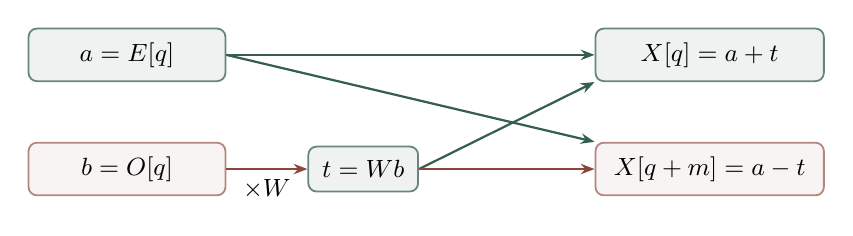
\begin{tikzpicture}
  \node[module,minimum width=25mm] (a) at (0,1.15) {$a=E[q]$};
  \node[module,minimum width=25mm,draw=BrickRed!65,fill=BrickRed!6] (b) at (0,-.3) {$b=O[q]$};
  \node[module] (t) at (3.0,-.3) {$t=Wb$};
  \node[module,minimum width=29mm] (plus) at (7.4,1.15) {$X[q]=a+t$};
  \node[module,minimum width=29mm,draw=BrickRed!65,fill=BrickRed!6] (minus) at (7.4,-.3) {$X[q+m]=a-t$};
  \draw[foldarrow] (a.east)--(plus.west);
  \draw[warmarrow] (b.east)--node[below] {$\times W$}(t.west);
  \draw[foldarrow] (t.east) -- (plus.south west);
  \draw[warmarrow] (t.east) -- (minus.west);
  \draw[foldarrow] (a.east) -- (minus.north west);
\end{tikzpicture}
\FigCap{图 1\quad 一只蝶形。相加与相减使用同一个旋转结果 $t$。}
\end{center}

单位根的模为 $1$，乘 $W$ 只改变 $b$ 在复平面上的方向，转角是 $-2\pi q/(2m)$。程序需保留旧的 $a$ 和 $t$，才能把两个结果写回同一对位置。

\FFTPage{三}{圆形折叠怎样配对}{disk}
\label{sec:disk}

把 8 个采样按 $0,1,\ldots,7$ 顺时针排到圆周。第 1 折把相隔半圈的 $j$ 和 $j+4$ 配起来，形成四个站点。每个站点对应一组长度为 2 的序列，先交给一个 2 点蝶形。

\begin{center}
\begin{minipage}[t]{.48\linewidth}\centering
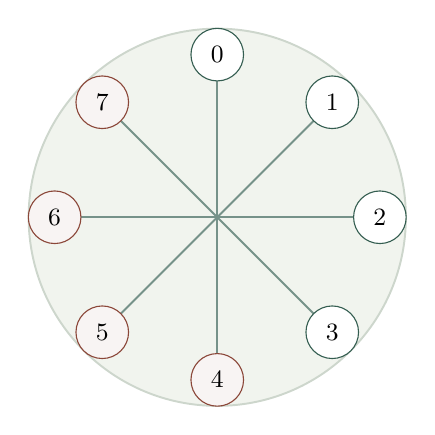
\begin{tikzpicture}[scale=1.18]
 \draw[disk,fill=InkWash] (0,0) circle (2.03);
 \foreach \j in {0,...,7} {
   \pgfmathsetmacro{\a}{90-45*\j}
   \coordinate (p\j) at (\a:1.75);
 }
 \foreach \j [evaluate=\j as \o using int(\j+4)] in {0,...,3} {
   \draw[foldchord] (p\j) -- (p\o);
 }
 \foreach \j in {0,...,7} {
   \ifnum\j<4
     \node[station] at (p\j) {$\j$};
   \else
     \node[warmstation] at (p\j) {$\j$};
   \fi
 }
\end{tikzpicture}
\par\small\color{handoutmuted}折前 · 圆周相对的两点配一组
\end{minipage}\hfill%
\begin{minipage}[t]{.48\linewidth}\centering
\begin{tikzpicture}[scale=1.18]
 \draw[disk,fill=InkWash] (0,0) -- (112.5:2.03)
      arc[start angle=112.5,end angle=-67.5,radius=2.03] -- cycle;
 \draw[disk,densely dashed] (0,0) circle (2.03);
 \foreach \j in {0,...,3} {
   \pgfmathsetmacro{\a}{90-45*\j}
   \pgfmathtruncatemacro{\o}{\j+4}
   \draw[foldchord] (0,0) -- (\a:1.75);
   \node[module,inner sep=2pt,font=\scriptsize] at (\a:1.77)
       {$\j,\textcolor{BrickRed}{\o}$};
 }
 \node[font=\small,text=RoyalBlue] at (-.24,-1.0) {$4$ 个站点};
 \node[font=\scriptsize,text=handoutmuted] at (-.24,-1.48) {每站两项};
\end{tikzpicture}
\par\small\color{handoutmuted}折后 · 编号 $j$ 保留，另一半叠过来
\end{minipage}
\FigCap{图 2\quad 8 点圆盘的第一次折叠。右图的数字是配在一起的原采样下标。}
\end{center}

\HandoutBlock{每个站点存什么}
长度为 2 时 $m=1$、$q=0$，因子 $\W_2^0=1$。因此第一折直接把两项的和、差写进站点。以 $j=1$ 为例，该站先接收 $x[1]$ 与 $x[5]$，再输出 $x[1]+x[5]$ 与 $x[1]-x[5]$。
\[
 \begin{array}{c|c|ll}
  \text{新站点 }j & \text{旧站点配对} & B_1[j,0] & B_1[j,1]\\ \hline
  0&(0,4)&x[0]+x[4]&x[0]-x[4]\\
  1&(1,5)&x[1]+x[5]&x[1]-x[5]\\
  2&(2,6)&x[2]+x[6]&x[2]-x[6]\\
  3&(3,7)&x[3]+x[7]&x[3]-x[7]
 \end{array}
\]

第 2 折时站点只剩 $0,1,2,3$，配对改为 $(0,2)$ 与 $(1,3)$。每对包含两个局部频点 $q=0,1$，分别做蝶形，把两份 2 点结果合成一份 4 点结果。第 3 折把最后两站合并，得到完整 8 点频谱。

\FFTNote{圆盘上移动半圈，让 $j$ 与 $j+d/2$ 落在同一站。复平面上乘 $\W_{2m}^{q}$ 负责旋转系数，其角度由 $q$ 决定。第一次折叠已经发生了配对，此时唯一的 $q=0$ 仍然对应零度数值旋转。}

\FFTPage{四}{每一折的不变量}{layers}
\label{sec:layers}

设总长度 $N=2^L$。折完 $s$ 次后，令 $m=2^s$、$d=N/m$。站点 $j$ 跟踪从 $x[j]$ 开始、每隔 $d$ 取一次的 $m$ 项子序列。状态矩阵的定义是
\begin{equation}
 B_s[j,q]=\sum_{r=0}^{m-1}x[j+rd]\,\W_m^{qr},
 \qquad 0\le j<d,\quad 0\le q<m.
 \label{eq:layer}
\end{equation}
每一行是一份独立的 $m$ 点 DFT，行与列的含义不同。行号 $j$ 决定从哪里取原采样，列号 $q$ 决定读哪个局部频点。

\HandoutBlock{从第 $s$ 层推出第 $s+1$ 层}
在 $s<L$ 时令 $d'=d/2$，新序列 $y_j[t]=x[j+td']$ 有 $2m$ 项。在任取的新站点 $0\le j<d'$，
\[
 \begin{aligned}
 y_j[2r]   &= x[j+rd],     &&\text{来自旧站 }j;\\
 y_j[2r+1] &= x[j+d'+rd],  &&\text{来自旧站 }j+d'.
 \end{aligned}
\]
这两个序列各有 $m$ 项。按式~\eqref{eq:layer}，它们的局部频点恰为 $a=B_s[j,q]$ 与 $b=B_s[j+d',q]$。把这两个数代入式~\eqref{eq:butterfly}。
\begin{align}
 t&=\W_{2m}^{q} B_s[j+d',q],\notag\\
 B_{s+1}[j,q]&=B_s[j,q]+t, \label{eq:layer-first}\\
 B_{s+1}[j,q+m]&=B_s[j,q]-t. \label{eq:layer-second}
\end{align}
每组结果的前半段按 $q$ 存放，后半段按 $q+m$ 存放。每次折叠后行数减半，列数翻倍，数据总量仍为 $N$。

\begin{center}
\begin{tikzpicture}
 \node[module] (s0) at (0,0) {$B_0$\\$8\times1$};
 \node[module] (s1) at (3,0) {$B_1$\\$4\times2$};
 \node[module] (s2) at (6,0) {$B_2$\\$2\times4$};
 \node[module] (s3) at (9,0) {$B_3$\\$1\times8$};
 \draw[foldarrow] (s0)--node[above] {\scriptsize 第1折}(s1);
 \draw[foldarrow] (s1)--node[above] {\scriptsize 第2折}(s2);
 \draw[foldarrow] (s2)--node[above] {\scriptsize 第3折}(s3);
\end{tikzpicture}
\FigCap{图 3\quad 8 点 FFT 的行列形状。每层恰好包含 8 个复数。}
\end{center}

当 $s=0$ 时 $m=1,d=N$，式~\eqref{eq:layer} 直接给出 $B_0[j,0]=x[j]$。当 $s=L$ 时 $d=1,m=N$，代入 $j=0$ 得 $B_L[0,k]=X[k]$，其转置就是输出列向量 $\bt{X}$。因此只要每一折满足式~\eqref{eq:layer-first} 与 \eqref{eq:layer-second}，最终结果就与定义式~\eqref{eq:dft} 相同。

\FFTPage{五}{四个采样，完整算两折}{worked}
\label{sec:four}

输入是 $(x[0],x[1],x[2],x[3])=(1,2,3,4)$。第 1 折对偶、奇两组分别取和与差。
\[
 E=\begin{bmatrix}1+3\\1-3\end{bmatrix}
   =\begin{bmatrix}4\\-2\end{bmatrix},
 \qquad
 O=\begin{bmatrix}2+4\\2-4\end{bmatrix}
   =\begin{bmatrix}6\\-2\end{bmatrix},
 \qquad
 B_1=\begin{bmatrix}4&-2\\6&-2\end{bmatrix}.
\]
$E,O$ 上面写为两个列向量，放进中间矩阵时分别转置为一行。第 2 折每次沿竖直方向取同一列的两个数。

\begin{tabularx}{\linewidth}{@{}cclY@{}}
\toprule
列 $q$ & 所取的一对 $(E[q],O[q])$ & $W=\W_4^q$ & 写入输出 \\
\midrule
$0$ & $(4,6)$ & $1$ & $X[0]=4+6=10$，$X[2]=4-6=-2$。 \\
$1$ & $(-2,-2)$ & $\ee^{-\pi\ii/2}=-\ii$ & 先得 $t=(-\ii)(-2)=2\ii$，再把 $-2+2\ii$ 写入 $X[1]$，把 $-2-2\ii$ 写入 $X[3]$。 \\
\bottomrule
\end{tabularx}

\begin{center}
\begin{tikzpicture}[scale=1.18]
  \draw[guideaxis] (-2.75,0)--(2.5,0) node[right] {$\operatorname{Re}$};
  \draw[guideaxis] (0,-.58)--(0,2.6) node[above] {$\operatorname{Im}$};
  \fill[handoutmuted] (0,0) circle (1.2pt);
  \draw[warmarrow,line width=1pt] (0,0)--(-2,0)
       node[below left,BrickRed] {$b=-2$};
  \draw[foldarrow,line width=1.05pt] (0,0)--(0,2)
       node[above right,RoyalBlue] {$t=2\ii$};
  \draw[warmarrow,densely dashed] (-.84,0) arc (180:90:.84);
  \node[font=\small,align=center] at (2.08,1.65)
       {$\times(-\ii)$\\[2pt]顺时针 $90^\circ$};
\end{tikzpicture}
\FigCap{图 4\quad 第 2 折的第 1 列。$-2$ 的方向从 $\pi$ 变成 $\pi/2$，长度仍是 $2$。}
\end{center}

两列的计算分别写入下标 $(0,2)$ 和 $(1,3)$，最终输出按 $k=0,1,2,3$ 排列。
\[
 B_2=\begin{bmatrix}10&-2+2\ii&-2&-2-2\ii\end{bmatrix},
 \qquad
 \bt{X}=B_2^{\rankff}.
\]

\FFTNote{先核对 $X[0]=1+2+3+4=10$。实输入的 $X[1]$ 与 $X[3]$ 互为共轭。若它们的虚部互换，先查正向指数的符号。}

\FFTPage{六}{把 FFT 写成矩阵乘积}{matrix}
\label{sec:matrix}

对长度 $2m$，令置换矩阵 $P$ 把自然顺序的输入重排为前半偶项、后半奇项。设
\[
 D_m=\operatorname{diag}(\W_{2m}^{0},\W_{2m}^{1},\ldots,\W_{2m}^{m-1})
       \in \Cplx^{m\times m}.
\]
用分块对角矩阵分别计算两份 $m$ 点 DFT，再以式~\eqref{eq:butterfly} 做两份向量的加减。于是
\begin{equation}
 F_{2m}=
 \underbrace{\begin{bmatrix}I_m&D_m\\I_m&-D_m\end{bmatrix}}_{M_{2m}}
 \begin{bmatrix}F_m&0\\0&F_m\end{bmatrix} P.
 \label{eq:matrix-factor}
\end{equation}
按从右到左的顺序，$P$ 配对，分块对角矩阵产生 $E,O$，$M_{2m}$ 将它们合并成自然频点顺序的 $X$。对角矩阵 $D_m$ 逐项乘奇组，对每个 $q$ 只访问同一个局部下标。

\HandoutBlock{把 4 点例子中的矩阵写开}
此时 $\W_4=-\ii$，$m=2$，$D_2=\operatorname{diag}(1,-\ii)$，所以
\[
 P_4=\begin{bmatrix}
 1&0&0&0\\0&0&1&0\\0&1&0&0\\0&0&0&1
 \end{bmatrix},
 \qquad
 F_2=\begin{bmatrix}1&1\\1&-1\end{bmatrix},
 \qquad
 M_4=\begin{bmatrix}
 1&0&1&0\\0&1&0&-\ii\\1&0&-1&0\\0&1&0&\ii
 \end{bmatrix}.
\]
实际的乘法顺序和两折对应如下。$v_1$ 是把 $B_1$ 的两行依次接到一起得到的列向量。
\[
\begin{aligned}
 v_0&=P_4\bt{x}=[1,3,2,4]^{\rankff},\\
 v_1&=\operatorname{diag}(F_2,F_2)v_0=[4,-2,6,-2]^{\rankff},\\
 \bt{X}&=M_4v_1=[10,-2+2\ii,-2,-2-2\ii]^{\rankff}.
\end{aligned}
\]
也可以直接乘完整的 DFT 矩阵验算。
\[
 F_4=
 \begin{bmatrix}
 1&1&1&1\\
 1&-\ii&-1&\ii\\
 1&-1&1&-1\\
 1&\ii&-1&-\ii
 \end{bmatrix},
 \qquad
 F_4\bt{x}=
 \begin{bmatrix}10\\-2+2\ii\\-2\\-2-2\ii\end{bmatrix}.
\]
例如取下标为 $k=1$ 的行，得到 $1-2\ii-3+4\ii=-2+2\ii$，正是第 2 折中 $q=1$ 的加法结果。

\FFTPage{七}{递归写法：沿步长取样}{recursive}
\label{sec:recursive}

下面的 C99 写法可以直接编译。输入指针 \texttt{x} 指向当前子序列首项，\texttt{stride} 表示相邻两项的间隔。调用者提供长度为 $N$、互不重叠的输入和输出缓冲区。入口从自然顺序读取，最外层取 \texttt{stride = 1}。输出也是自然顺序。代码共用 \texttt{<complex.h>} 和 \texttt{<stddef.h>}，$I$ 在代码中是虚数单位。

\lstinputlisting[firstline=4,lastline=14]{fft.c}
\lstinputlisting[firstline=16,lastline=42]{fft.c}

\HandoutBlock{逐句对照}
{\small\noindent
\begin{tabularx}{\linewidth}{@{}lY@{}}
\toprule
代码中的动作 & 数学含义 \\
\midrule
\texttt{n == 1} & 单点变换等于该点本身。 \\
\texttt{x}, \texttt{x + stride} & 偶子序列和奇子序列的首地址。两次调用的步长都翻倍。 \\
\texttt{out}, \texttt{out + m} & 前 $m$ 格存 $E$，后 $m$ 格存 $O$。 \\
\texttt{a}, \texttt{t} & 先保存 $E[q]$，再算 $Wb$。写回前两项都已读出。 \\
两次写回 & 对应式~\eqref{eq:butterfly} 的 $q$ 位与 $q+m$ 位。 \\
\bottomrule
\end{tabularx}\par}

\FFTPage{八}{迭代写法：位反转后原地合并}{iterative}
\label{sec:iterative}

递归先依据二进制下标的最低位拆偶、奇，再依据更高一位继续拆。按叶节点从左到右读取时，低位成了外层顺序。把下标的 $L$ 个二进制位反过来，就得到这个访问次序。4 点时 $\texttt{00},\texttt{01},\texttt{10},\texttt{11}$ 反转后为 $\texttt{00},\texttt{10},\texttt{01},\texttt{11}$，数组先变成 $[1,3,2,4]$。

\lstinputlisting[firstline=44,lastline=81]{fft.c}

\HandoutBlock{合并块的读法}
\texttt{len} 是当前待合成的长度，\texttt{m = len / 2}。每个块从 \texttt{start} 开始，前半和后半各有一份已完成的 $m$ 点变换。第 $q$ 次配对读 \texttt{u = start + q} 与 \texttt{v = u + m}，乘的单位根是当前长度的 $\W_{\texttt{len}}^q$。长度为 $2,4,\ldots,N$ 的各层处理完以后，数组就是自然频点顺序的 $X$。

\FFTPage{九}{复杂度、逆变换与验算}{verify}
\label{sec:verify}

\HandoutBlock{为什么运算量是 $N\log_2N$}
同一层的 $d$ 个站点分成 $d/2$ 对。每对有 $m$ 个局部频点，每个频点一次蝶形，因此每层有 $(d/2)m=N/2$ 只蝶形。每只蝶形至多一次复乘、两次复加减，共 $\log_2N$ 层。
\[
 \#\text{蝶形}=\frac{N}{2}\log_2 N,\qquad
 T(N)=2T(N/2)+\Theta(N)=\Theta(N\log N).
\]
4 点用 4 只蝶形，32 点用 80 只蝶形。直接 DFT 对每个频点逐项累加，总代价是 $\Theta(N^2)$。递归版除了输入输出缓冲区，还用 $\Theta(\log N)$ 层调用栈。迭代版的数组原地更新，只另用常数个临时量。迭代位反转里的进位会翻转若干位，所有下标合计只翻转 $O(N)$ 次，因为从最高位向下以 $0$ 编号，第 $j$ 位每 $2^j$ 步翻转一次。

\HandoutBlock{复用正向程序来做逆变换}
对式~\eqref{eq:idft} 取共轭，可以把正指数换回负指数。数组先共轭，做正向 FFT，结果再共轭并除以 $N$。
\[
 \operatorname{IFFT}(\bt{X})=
 \frac{1}{N}\,\overline{\operatorname{FFT}(\overline{\bt{X}})}.
\]
源码中的 \texttt{ifft\_inplace} 执行这个过程。包内的测试独立地按 DFT 定义求和，并核对 4 点例题、长度 $1$ 到 $256$ 的 108 组复数输入、两种正向程序，以及正反变换往返。

\HandoutBlock{自己再检查三处}
\begin{enumerate}
 \item 从 $\W_{2m}^{q+m}=-\W_{2m}^{q}$ 推出蝶形的减号，指出代码里哪两行使用同一个 $t$。
 \item 把 8 点的第一次折叠写成 4 行 2 列。然后只追踪新站 $j=0$，写出第 2 折选取的四个原采样下标。核对点是 $0,2,4,6$。
 \item 输入常量序列 $[1,1,1,1]$，先手算再试代码。预期只在 $k=0$ 读到 $4$，其他项为零。
\end{enumerate}

\HandoutBlock{符号约定与延伸阅读}
实序列有共轭对称性。网页上的单边幅度谱会对 $|X[k]|/N$ 做归一化，对 $0<k<N/2$ 的项再乘 $2$。它与讲义和代码返回的复数频谱 $X[k]$ 使用不同标度。

{\small\color{handoutmuted}
\href{http://yeyaozhi.eu.cc/learning/math-lab/fft/}{数学实验室 · FFT 折叠实验} 提供相同的 4 点跟算和 32 点圆盘。\\
J. W. Cooley and J. W. Tukey,
\href{https://doi.org/10.1090/S0025-5718-1965-0178586-1}{An Algorithm for the Machine Calculation of Complex Fourier Series},
\emph{Mathematics of Computation} 19 (1965), 297--301。本讲义采用负指数的正向 DFT 约定。}
\end{document}
